%!TEX root = ../dissertation.tex
\clearpage
\section{microRNA Family Gene Ontology Enrichment}
A significant drawback of the recency of the discovery of regulatory small RNAs is the lack of comprehensive functional annotation. While protein coding genes are well annotated and neatly organised into an enormous amount of ontological categories (see Section \ref{sec:database:gsea}), \acp{mir} have only been anecdotally associated with specific functions in the cell. Additionally, the functional roles of protein coding genes are much more limited than those of \acp{mir}; the number of potential functions of any \ac{mir} correlates with the number of mRNA targets this \ac{mir} has, and is also highly context-dependent (e.g. regarding cell type, cell state, disease). Thus, to systematically screen a large amount of \acp{mir} and families, we had to turn to an indirect approach: the \ac{go} analysis of targeted genes.

\begin{method}

\subsection{microRNA Family Enrichment}
To categorise and systematise the sexual dimorphism of \ac{cntf} differentiation of LA-N cells, statistically over-represented \ac{mir} families in the differential expression datasets were determined. Of the 151 \ac{mir} families listed in miRBase v21, members of 71 families are \ac{de} in \ac{la2} and \ac{la5}. Enrichment of male, female, and ubiquitously \ac{de} \acp{mir} in these families was determined by hypergeometric enrichment via Fisher's exact test for each of the families. The targets of all individual \acp{mir} in the enriched families were determined via \textit{miRNeo} query. 

\subsection{Creation of miRNA Family Gene Target Sets}
\ac{go} analysis of the targets of a single \ac{mir} is challenging, because the analysis requires a weighted scoring system of input genes. For single \acp{mir}, the options for scoring are limited to the aggregated targeting score or permutation p-values. Using families enables the introduction of a further scoring method: the aggregation of individual family members targeting the same gene. The reasoning behind this approach is to determine a general functional »area« of biological process that the \ac{mir} family in question operates in. To account for the possibility of multiple areas being affected by a family, the test set of genes in any \ac{go} enrichment analysis should not be too small (i.e., rather the top 100 genes than the top 10). 

Following this reasoning, the targets of all \acp{mir} in each family were determined via \textit{miRNeo} query. For each family, genes were ranked by their cumulative targeting score $\rho$ from all family members. For gene $i$ and number of \acp{mir} in family $x$, gene score $\rho$ is calculated from individual \ac{mir}$\to$gene scores $s$: $$\rho_{i} = \sum_{n=1}^{x} s_{ni}$$

\subsection{GO Analysis of Target Sets} \label{sec:cellculture:topgo}
The gene target sets of individual \ac{mir} families were ordered decreasingly by their cumulative score $\rho$ and subjected to \ac{go} analysis via the R package \textit{topGO}.\cite{Alexa2006} Briefly, \textit{topGO} analysis extends the basic hypergeometric approach of \ac{go} enrichment analysis by de-correlating the \ac{dag} structure of GO annotation (see Section \ref{sec:database:gsea}), allowing a weighted correction for the interdependency of neighbouring GO nodes. If a gene is found in both the parent node (more general) and the child node (more specific), the less specific parent node gene is weighted less; in this way, the most specific node of each hierarchical branch can be found without confounding the result with less specific terms. While GO analysis always is subject to interpretation by the researcher, this weighted algorithm has been shown to reduce false positives while retaining a high true positive ratio.

\textit{topGO} analysis was performed using the classic (i.e., Fisher's exact test) as well as weighted methods for comparison, however, to determine significance, the p-values calculated by the enhanced weighted algorithm were used. \ac{fdr} was controlled at 5\%. As recommended by the authors,\cite{Alexa2006} the ordered list of gene targets up to the 3000th position was used as a background for the analysis; the test set in each case was the top 10\% of targeted genes.

\end{method}

\subsubsection{Gene Targeting of Enriched Families}
Five families were enriched in both male and female cells, and 12 families in only one of the two cell lines (Fig.\,\ref{fig:mir-de-fam-go}\,A, left side). The size range of enriched families was substantial, from small families with only 4 mature members to extensive families with dozens of mature \acp{mir}. Of note, the amount of family members in any \ac{mir} family did not correlate with the absolute amount of targets predicted (Fig.\,\ref{fig:mir-de-fam-go}\,A). Rather, the influence of individual \acp{mir} was the main factor determining the size of the gene target network. However, those families that were enriched in only one cell line presented with significantly smaller target sets than those that were found \ac{de} in both (mean targeted genes per \ac{mir} 217 versus 378, Welch two-sample t test, p = 0.001). Relative to family size, 4 of the enriched families targeted less genes than all others: mir-10 (p = 0.016), mir-192 (p = 0.042), mir-379 (p = 0.011), and mir-515 (p < 0.001). Hypothetically, the spectrum of target amounts may correlate with the degree of functional specification of distinct \ac{mir} families: on one end, broadly acting families such as let-7 with sex-independent function, on the other, families with a narrow target profile, such as mir-10, whose restricted function can associate with sex-specific effects.

\begin{figure}
\centering
\includegraphics[width=\textwidth]{figures/mir-de-fam-go}
\caption[Differential Expression miRNA Family Enrichment]{\textbf{miRNA Families Enriched in Differential Expression and their Ontological Associations.} 17 miRNA families were enriched significantly in the DE miRNAs following CNTF-mediated differentiation of LA-N-2 and LA-N-5 (Fisher's exact test, p < 0.05). \textbf{A, left side)} Bar plot of p-values of enriched families, ordered by family size; family size encoded by colour. \textbf{A, right side)} Stacked bar plot of the number of gene targets per family. Bars are divided by the DE pattern between LA-N-2 and LA-N-5 of each individual family member. DE context (encoded by colour) varies from detection in all categories (such as let-7 or mir-10) to detection only in one cell line (such as mir-515 or mir-154). Four families show significantly less target genes than all other families in relation to their size (denoted by asterisks). \textbf{B)} Gene Ontology enrichment analysis of gene targets of all enriched families via 737 distinct terms curated into CNS- or immunity-related categories. The miRNA families mir-10 and mir-199 show association with neurokines and circadian rhythm.
\label{fig:mir-de-fam-go}}
\end{figure}

\subsection{Large Scale GO Term Curation}
The GO analysis performed in this manner for all 17 enriched families resulted in a list of 737 distinct GO terms related to any of the families. To generate an overview of functional implications of the individual families, the GO terms were filtered and aggregated manually. Terms not relating to CNS- or immune-function were removed, and the remaining terms were sorted into one of 21 categories (Fig.\,\ref{fig:mir-de-fam-go}\,B). Generally, the 17 miRNA-families associate with neurodevelopment and neural plasticity, diverse immune functions, cell cycle control, and sex. Most families present with association to general ontological categories such as neurodevelopment or sex, while more specific categories show a sparser distribution.

Only two families associate significantly with neurokine-related function, mir-10 and mir-199. Both are, as many others, involved in neurodevelopment- and sex-related function, but both also show the very specific association with circadian rhythm. Family mir-10 additionally is implicated in control of neurotrophin-related mechanisms, and in several blood-borne immune cells, such as T-, B-, and NK-cells.

\section{Whole Genome miRNA$\to$Gene Network Generation} \label{sec:cellculture:network}
A common approach to complex network relationships is physical modelling. A complex graph (with directed and weighted edges) can be coerced to self-organise by application of a force-directed layout. In this process (also known as spatialisation), the network, defined only by its nodes and edges, is transformed into a map, usually in two dimensions. An important prerequisite is the scale-free topology of the network, a structure that transcriptional connectomes usually present with.\cite{Broido2019} A force-directed layout transforms a network by simulating a gravitational system, or a system of magnetic nodes connected by springs, in which the nodes repel each other, but edges between two nodes pull them towards each other. By manipulation of multiple physical attributes of the model, a mapped representation of the network's organisation can be produced. As a result, nodes (i.e., genes, TFs, and miRNAs) with close interaction are mapped in close proximity, while nodes with low interaction are far apart. Similarly, nodes with pivotal function in the network (»hubs«) gravitate towards the centre of the map, while »less important« nodes are shifted towards the fringes.

\begin{method}

The network comprising all \ac{de} members of the 17 enriched miRNA families and \num{12495} targeted genes as determined via \textit{miRNeo} query was subjected to force-directed mapping using the Java-based software Gephi 0.9 and its primary force-directed algorithm, ForceAtlas2.\cite{Jacomy2014} Gephi, and ForceAtlas2, are designed to generally handle graphs with up to \num{10000} unique relationships; however, the standard \textit{miRNeo} query resulted in a network with $\smallsim$\num{160000} edges. To reach a computationally manageable number of relationships, the score threshold was raised to a minimum of 7, which resulted in a network of \num{46937} unique edges. The resulting network was exported as a vector graph and manually edited in Adobe Illustrator to further enhance its readability (Fig.\,\ref{fig:bignet}).

\end{method}

\begin{figure}
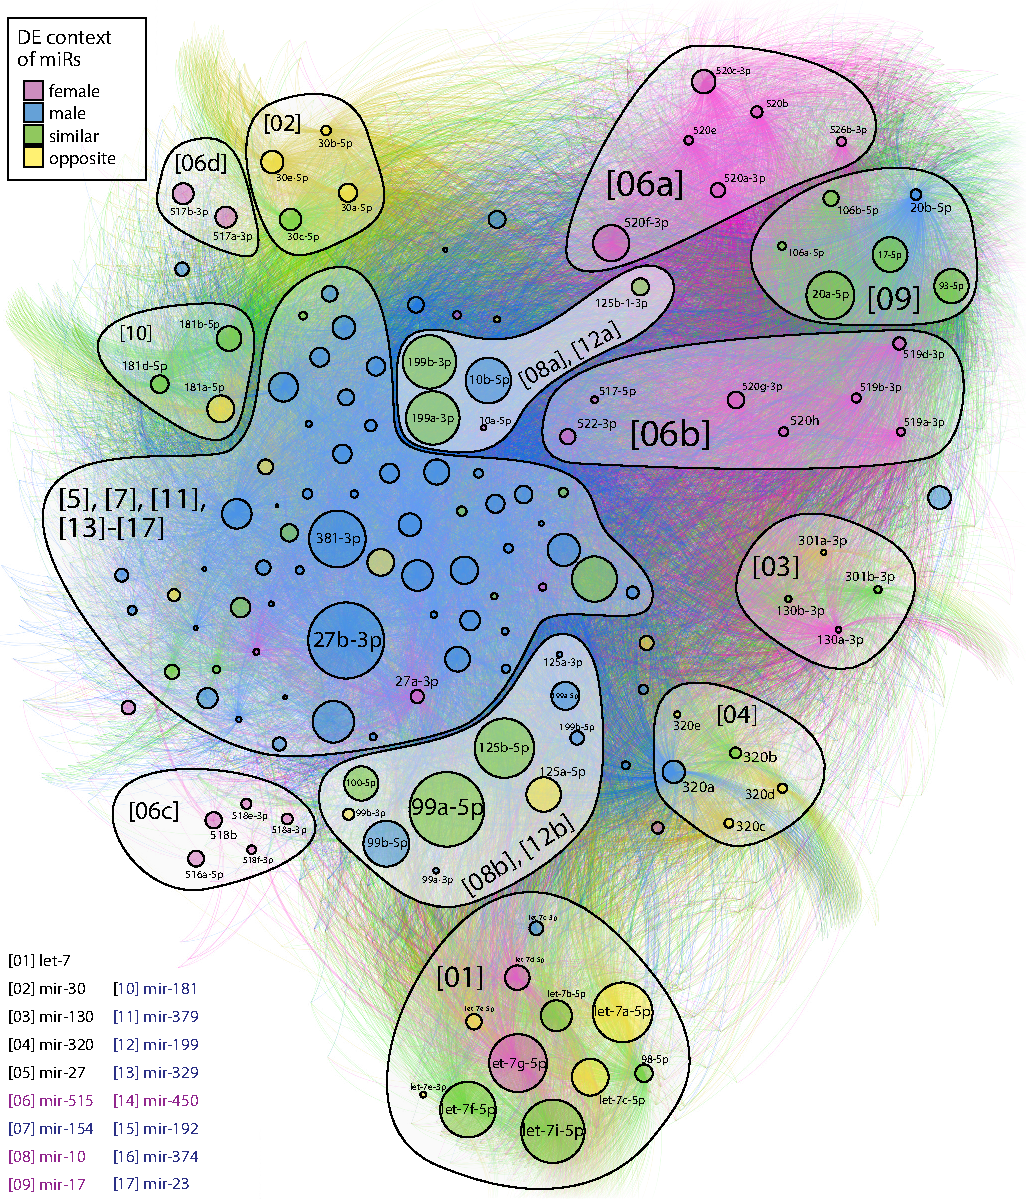
\includegraphics[width=\textwidth]{figures/bignet}
\caption[LA-N-2 / LA-N-5 Full Connectome.]{\textbf{Full Connectome of LA-N-2 and LA-N-5 Differentially Expressed miRNA Families.} The network of miRNA families and their \num{12495} targeted genes self-organises into a connectome map with \num{46937} unique edges. miRNA node size scaled by absolute count-change, nodes coloured by DE context. Numbers in brackets denote miRNA families, gene nodes have minimal size. By application of a force-directed layout, the miRNA families visibly self-segregate into clusters. The let-7 family, male-biased and female-biased clusters take up major parts of the network. Families mir-10 and mir-199, with neurokine association, form two mixed, sexually dimorphic clusters near the centre of the map (lighter shade).
\label{fig:bignet}}
\end{figure}

The resulting transcriptional connectome map illustrates the functional compartmentalisation of miRNA$\to$gene interactions. miRNAs of distinct families are frequently found in close proximity to one another, most often forming one or two clusters. In the case of two clusters forming, the clusters are usually representative of the two complementary strands of the pre-miRNA(s), since 3' and 5' variants of any pre-miRNA usually possess fundamentally different seed sequences, and thus, targets. The let-7 family is distinguished by its removal from the bulk of other interactions, possibly representing a particularly specialised set of functions, at least for the 5' variants of the bottom cluster\todo{evolutionary? discussion?}. Families with predominant differential expression in one of the two cell lines (sexes) inhabit different sides of the main graph and show little intermingling, pointing towards sexually dimorphic gene target distribution. The two neurokine-associated families, mir-10 and mir-199, are located near the centre of the graph, in two strand specific clusters (»[08a]\&[12a]« and »[08b]\&[12b]«).

To gather more detailed information than grouping of miRNAs with similar function, such as direct miRNA$\to$gene interaction, the size of the studied networks must be reduced. For each family affected by CNTF-differentiation, a single graph was created, laid out by application of ForceAtlas2, and analysed for critical nodes. The distinct families and their gene targets yield immensely diverse graph layouts, that here cannot be described in their entirety. However, the entire collection of graphs in interactive visual form is accessible at \url{https://slobentanzer.github.io/cholinergic-neurokine}. Due to an elevated interest, the cholinergic/neurokine miRNA interface and the families mir-10 and mir-199 will be described in more detail, and in conjunction with sex-specific perturbations in neurologic diseases.

\newpage

%\section{The Cholinergic/Neurokine Interface}
%
%\begin{method}
%
%\subsection{Network Generation}
%To the set of cholinergic genes (see Box \ref{box:chol-genes}) were added: the genes for neurokines and their receptors, second messenger pathways (most importantly JAK/STAT), neurotrophin-related genes, and circadian genes.
%\todo{network of cholinergic/neurokine? mirs? both?}
%\todo{mir-125 ache culture test?}
%\todo{adjacency by targeted genes?}
%
%\end{method}
